\section[Integral geometry. Or ``How long is a piece of string?'']{Integral geometry\\ {\large Or ``How long is a piece of string?''}}
\label{sec:integral-geometry}

\subsection{Towards a geometric interpretation of extensivity}

Geometry has been a recurring theme in physical theories, appealing because of its intuitive nature.
There are many ways that geometric ideas can be incorporated, but our focus will be on expansions of thermodynamic quantities in terms of \emph{sizes}.
The usefulness of this particular focus is directly connected to the familiar concept of \emph{extensivity} in statistical mechanics, which we will use to guide the following discussion.
Thermodynamic potentials must be extensive to remain well-defined in the thermodynamic limit,
%Defining an extensive quantity as one that scales proportionally to system size, the first meaning of size that comes to mind is probably the volume.
so by focusing on extensive quantities we ensure a thermodynamically consistent description in this limit.

%The first notion of size that likely comes to mind is the volume, though we will generalise to all reasonable notions of size.
%The simplest example we can give is from statistical mechanics: an \emph{extensive variable} is one that scales proportionally to the system volume.
%For a finite system $K \subset \mathbb{R}^d$ %the volume is expressed
%% \begin{equation}
%%   V[K] = \int_K d\vec{r}.
%% \end{equation}
%Then,
As an example, extensive quantities include the \emph{potential energy} of a large system which can be expressed in terms of system volume as
\begin{equation*}
  \lim_{V \to \infty} U = u V
\end{equation*}
where $u$ would be an energy density which is \emph{intensive}, meaning it does not change with system volume.
Another example is the surface free energy, defined in the absence of entropic effects as the excess quantity $U_\mathrm{ex} = U - uV$
In the macroscopic limit this yields the extensive quantity
\begin{equation*}
  \lim_{V \to \infty} U_\mathrm{ex} = \gamma A
\end{equation*}
where $\gamma$ is the intensive surface tension and $A$ is the extensive surface area i.e.\ another size measure.
More refined notions define a variable as extensive if it is a \emph{first-order homogeneous function} of any linearly independent set of (different) extensive variables characterising the system size \cite{Chandler1987}.
That is, a variable $\phi$ is extensive if
\begin{equation}\label{eq:extensive-homogeneity}
  \phi(\lambda Y_1, \cdots, \lambda Y_n)
  =
  \lambda \phi(Y_1, \cdots, Y_n)
\end{equation}
where $\{Y_1, \cdots, Y_n\}$ are a complete (linearly independent) set of extensive variables describing the system size.
We will explore what other reasonable notions of `size' there may be, in effect finding a complete set of extensive variables, in the hope that we arrive at ideas which prove useful in developing new theories.

We introduced the area above as a size descriptor for a surface.
Borrowing ideas from differential geometry, we can also characterise the surface's shape through \emph{curvature}.
A surface is a two-dimensional manifold so its local shape is described by two basis vectors.
Supposing the surface is parameterised by coordinates $(x_1, x_2)$, then the basis vectors at a point on the surface $\vec{r}$ are
\begin{equation}
  \vec{e}_\alpha := \frac{\partial \vec{r}}{\partial x_\alpha}
  \qquad \alpha \in \{1, 2\}.
\end{equation}
Then, the shape of the surface is characterised by changes in the basis vectors leading to the curvature tensor
\begin{equation}
  \kappa_{\alpha \beta} := \frac{\partial \vec{e}_\beta}{\partial x_\alpha}
  \qquad \alpha, \beta \in \{1, 2\}.
\end{equation}
The values of the curvature tensor will depend on the choice of coordinate system $(x_1, x_2)$, so it is usual to consider the \emph{curvature invariants}, i.e.\ the trace and determinant%
\marginfootnote{This argument is readily generalised to $(d-1)$-dimensional surfaces in $\mathbb{R}^d$, where we would find $d-1$ invariants of the curvature tensor.},
leading to the the \emph{mean} and \emph{Gaussian curvatures}
\begin{subequations}
  \begin{align}
    H &:= \frac{\Tr{\kappa}}{2}, \\
    G &:= \det{\kappa}.
  \end{align}
\end{subequations}
As an example of how curvature can be a useful concept in statistical mechanics, we put forward the Young-Laplace equation which writes the pressure difference between two fluids as
\begin{equation*}
  \Delta p = 2 \gamma H,
\end{equation*}
with applications to e.g.\ phase coexistence \cite{YoungPTRSL1805,Laplace1805} or frost damage to porous solids \cite{EverettTFS1961}.
Extensive curvature measures are obtained by integrating the curvature invariants over the surface, leading to the integrated mean and Gaussian curvatures $C$ and $X$.

Together, the extensive geometric variables we have introduced so far can be written as%
\marginfootnote{We use the usual physicist abuse of notation where $V$ refers to both a region in space $V \subset \mathbb{R}^3$, and also the physical volume of this space.}
\begin{subequations}\label{eq:intrinsic-volumes-surface-integrals}
  \begin{align}
    \label{eq:volume-measure}
    V
    &=
    \int_V \, d\vec{r},
    \\
    A
    &=
    \int_{\partial V} \, d\vec{r},
    \\
    C
    &=
    \int_{\partial V} H(\vec{r}) \, d\vec{r},
    \\
    X
    &=
    \int_{\partial V} G(\vec{r}) \, d\vec{r}.
  \end{align}
\end{subequations}
The latter three quantities are \emph{expressed} here as the surface integrals, but we shall see that they are really size measures on the volume $V$.
These clearly form a linearly independent set%
\marginfootnote{This can be quickly determined by considering their units, i.e.\ $V: [\si{\metre^3}]$, $A: [\si{\metre^2}]$, $C: [\si{\metre^1}]$, $X: [\si{\metre^0}]$.},
but less obvious is the fact that these are the \emph{only} reasonable notions of size in three-dimensions.
This is a central finding of \emph{integral geometry}, which we will expand on in subsequent sections.
%is a powerful tool for incorporating intuitive, flexible ideas into theories.
%For this reason geometric approaches are common in statistical mechanics such as the Young-Laplace equation, which corrects Asakura-Ozawa
A consequence of this is that together $\{V, A, C, X\}$ form a complete basis for system size in three dimensions, so we could redefine an extensive quantity as one which can be written
\begin{equation}\label{eq:extensive-integral-geometry}
  \phi = a_3 V + a_2 A + a_1 C + a_0 X,
\end{equation}
which, as a linear relation, clearly obeys \eqref{eq:extensive-homogeneity} during the transformation%
\marginfootnote{Note: the rescaling of $\lambda V$ here refers to rescaling the volume measure \eqref{eq:volume-measure}, \emph{not} the object $V \subset \mathbb{R}^3$; in the latter case we would obtain the (non-extensive) transformation $\{V, A, C, X\} \to \{\lambda V, \lambda^{2/3} A, \lambda^{1/3} C, X\}$.}
$\{V, A, C, X\} \to \{\lambda V, \lambda A, \lambda C, \lambda X\}$.

Integral geometry provides elegant and unified description of sizes, and was crucial in the development of modern theories of hard spheres \cite{RosenfeldPRL1989,KonigPRL2004}, including the main ideas underlying chapters \ref{chapter:morphometric-framework}, \ref{chapter:morphometric-applications} and \ref{chapter:resummation}.
This framework thus provides the route to generalising geometrical theories such as the Asakura-Oosawa model for depletion forces \cite{AsakuraJCP1954,AsakuraJPS1958}, and more generally any free volume theory which expresses an energy in terms of a volume in space.
%Integral geometry generalises the underlying geometric principles of these theories into a unified framework for characterising size.
%% We could argue that fundamentally these theories are based on measuring physical sizes.
%% Integral geometry offers a mathematically rigorous formalism for describing sizes, so presents a possible starting point for free volume theories.
%Ideas from this branch of mathematics were crucial to the development of fundamental measure theory (section \ref{sec:fmt}), so it makes sense to place this before the section on liquid state theory.
As integral geometry is generally unfamiliar to people with a background in physics, we will place emphasis on the concepts and intuition rather than rigour and proofs.
We work mainly from standard texts Refs.\ \cite{Santalo2004,SchneiderACIG1984,Schneider2008,Klain1997}.

\subsection{What do we even mean by size?}
\label{sec:what-is-size}

In order to proceed we must define `size', and specify precisely which objects this definition applies to.
We put forward the following qualities of the measures $V, A, C$ and $X$ which make them intuitive notions of size:
\begin{enumerate}
\item They are invariant with respect to translations and rotations, so that an object's size is independent of the observer.
\item They increase additively, i.e.\ they transform under combination of subsystems via the inclusion/exclusion relation e.g.\ for two objects $K_1$ and $K_2$%
  \marginfootnote{We use the square brace notation $V[\cdot]$ to indicate that the size measures are generalised functions, or \emph{functionals}, of their arguments.}
  \begin{equation}\label{eq:additivity}
    V[K_1 \cup K_2] = V[K_1] + V[K_2] - V[K_1 \cap K_2],
  \end{equation}
  and similar expressions for $A$, $C$, and $X$.
  As corollaries, this property contains the idea that the size of nothing is zero, e.g.\ $V[\emptyset] = 0$, and leads to the homogeneity property of extensive variables \eqref{eq:extensive-homogeneity} through \eqref{eq:extensive-integral-geometry}.
\item They are continuous%
  \marginfootnote{Specifically, in integral geometry this continuity property is with respect to the \emph{Hausdorff metric}.
    Details on this can be found in standard texts, e.g.\ Refs.\ \cite{Santalo2004,SchneiderACIG1984,Schneider2008,Klain1997}.}.
  Loosely speaking, this means that the size measures converge as the object is approximated by increasingly finely meshed polyhedra excluding fractal geometries.
  As a simple intuitive example, the measurement of a length will converge continuously to some number as one uses rulers with progressively finer distance markings.
\end{enumerate}
The final property specifically excludes geometries for which we do not expect there to be any reasonable measurement of size.
These properties are the defining characteristics of more general size measures in integral geometry \cite{Santalo2004, Klain1997}.

%% First we define our objects: sets in Euclidean space.

%% We could completely describe the size of simple objects by completely defining their geometry, e.g.\ the dimensions of a box.
%% This is of course sufficient, however it is not very useful.
%% However, this may not be straightforward for more complex objects, and by abstracting the problem somewhat we can obtain useful theorems etc.
%% We now give a brief justification of the above \emph{ansatzes}, in particular why there are only four terms in the expansion.
%% Radius is the only natural parameter for a sphere, however for more general geometries there might be arbitrarily many parameters so one may wonder if they should be included in a general geometric expansion.

Naively, we might attempt to evaluate the size measures on all subsets $V \subset \mathbb{R}^3$, however this turns out to be too broad a definition.
In particular, this leads to the \emph{Banach-Tarski paradox} in which an object can be broken into two, then recomposed through rigid transformations into two objects identical to the original one  \cite{BanachFM1924}; by \eqref{eq:additivity}, a paradox ensues where the original volume is equal to twice itself.
A better definition is the restriction to \emph{polyconvex sets}%
\marginfootnote{The set of polyconvex objects is also sometimes called the \emph{convex ring}.}: objects formed by countable union of \emph{compact} and \emph{convex} objects.
By compact, we mean objects which are
\begin{enumerate}
\item \emph{bounded}, so they must be finite in scope, as no meaningful size can be defined for a body spanning an infinite region of space, and
\item \emph{closed}, so they contain their boundary.
  %, so the surface exists on which measures $\{A,C,X\}$ are defined.
  %This is an important property which we will see by example in discussing the Gauss-Bonnet theorem below.
\end{enumerate}
We write the collection of objects in $d$-dimensions which are compact and convex as $\mathcal{K}^d$.
This class of objects covers most physically relevant geometries, excluding geometries where size measures may be pathological such as those with fractal structures.
%The empty set $\emptyset$ is a compact body, albeit a special case with zero size.
%Compact convex set $K \in \mathcal{K}$ notation.

%% The first intuitive notion for a size: the size of nothing is zero, i.e.:
%% where $\emptyset$ is the empty set.
%% A box: take the largest length, but then the `size' is not increased by modifying its smallest dimensions.
%% Ideally, we want a size measure that increases monotonically as we add additional material. This leads to additivity:
%% \begin{equation}
%%   \phi(A \cup B) = \phi(A) + \phi(B) - \phi(A \cap B)
%% \end{equation}
%% Connection with entropy, leads to homogeneity in arguments which is the building block for extensivity of a thermodynamic potential.
%% This provides a geometrically precise foundation for thermodynamic potentials.

As a way of justifying the above claims, and as a segue into other topics, we introduce a (seemingly) new measure: the \emph{Euler characteristic} $\chi$ which simply counts the number of disjoint objects in a set%
\marginfootnote{As an intuitive illustration of why this is a size measure, I like to imagine that the \emph{size} of a pirate's treasure is the \emph{number} of gold coins in their possession, which is the Euler characteristic of their hoard.}.
More precisely, for a compact and convex object $K \in \mathcal{K}^d$ we define the measure such that
\begin{equation}\label{eq:euler-characteristic-definition}
  \chi[K] :=
  \begin{cases}
    1 & \textrm{if } K \ne \emptyset \\
    0 & \textrm{if } K = \emptyset
  \end{cases}
\end{equation}
then for it to behave additively \eqref{eq:additivity} for a disjoint collection of objects $K_1, \cdots, K_N \in \mathcal{K}^d$ with $K_i \cap K_j = \emptyset$ for $i \ne j$ we find
\begin{equation*}
  \chi[K_1 \cup \cdots \cup K_N] = N,
\end{equation*}
so it is a counting measure.
Some modification of its definition as a counting measure is needed in case of overlaps, however for now we focus on the fact that this measure is rigid-motion invariant, additive and continuous; as such, it would seem to be an independent measure.
However, the \emph{Gauss-Bonnet theorem} from differential geometry equates it with the Gaussian curvature through
\begin{equation}\label{eq:gauss-bonnet}
  X[K] = 2\pi \chi[\partial K],
\end{equation}
so it is really a manifestation of a size measure we have already seen.
It is worth emphasising the Euler characteristic in its own right however, as it is a very important \emph{topological invariant} meaning it does not change with continuous geometric deformations.
We state some important properties of the Euler characteristic below.

Compact objects include their boundary, so using the additivity property we can decompose the Euler characteristic on $K \in \mathcal{K}^d$ into surface and interior terms
\begin{equation*}
  \chi[K] = \chi[ \partial K ] + \chi[ \interior(K) ] = 1.
\end{equation*}
Arguing by induction, we find%
\marginfootnote{Briefly, the only compact, convex object in $d=1$ is a line segment, with $\partial K$ formed by two disjoint points giving $\chi[\partial K] = 2$.
  Then, in arbitrary dimensions one considers cutting the object in two, leading to an iteration formula which gives the stated result.
  Full details can be found in Ref.\ \cite{Klain1997}.}
\begin{subequations}
  \begin{align}
    \chi[ \partial K ] &= 1 + (-1)^d
    \\
    \chi[ \interior(K) ] &= (-1)^{d+1}
  \end{align}
\end{subequations}
Thus the Gauss-Bonnet theorem \eqref{eq:gauss-bonnet}, valid in $d=3$, gives $X = 4\pi$ for convex objects i.e.\ a constant.
By similar arguments, it can be shown that the Euler characteristic is increased by the number of \emph{cavities} in $K$, and decreased by the number of \emph{holes} in $K$ \cite{Klain1997}.
More generally, the Euler characteristic is modified by $(-1)^{\nu+1}$ times the number of $\nu$-dimensional \emph{voids}.

%% Repeat arguments in figures and you obtain the general rule that dividing an $n$-sphere gives two $n-1$-dimensional convex objects and a $n-1$ sphere dividor.
%% This gives us the rule for the Euler characteristic.
%% Euler characteristic describes the topology.

%% \begin{SCfigure}[H]
%%   \missingfigure[figwidth=0.5\linewidth]{$\partial B$}%
%%   \missingfigure[figwidth=0.5\linewidth]{$\partial B$}
%%   \caption{Effect of holes: divide 2d circle in two (2 rods + 2 points).}
%% \end{SCfigure}

%% \begin{SCfigure}[H]
%%   \missingfigure[figwidth=0.5\linewidth]{$\partial B$}%
%%   \missingfigure[figwidth=0.5\linewidth]{$\partial B$}
%%   \caption{Effect of cavities: divide 3d sphere in two (2 discs + circle).}
%% \end{SCfigure}

Having defined what we mean by `size', we can start to introduce some useful results from integral geometry.
This will start with generalisations of the size measures, and their completeness as a vector space for an extensive property \eqref{eq:extensive-homogeneity}.
Then, we will introduce formulae which are useful in evaluating partition functions for hard particle systems.

\subsection{Intrinsic volumes as generalised size measures}
\label{sec:generalised-intrinsic-volumes-d}

It will sometimes be helpful to use a dimension independent formalism%
\marginfootnote{Specifically, in chapter \ref{chapter:resummation} we will derive a theory for the liquid state.
  In order to obtain results for all physical dimensions $d \le 3$, we will work in arbitrary $d$ and substitute $d \in \{1, 2, 3\}$ at the end of our derivation.},
so it is convenient to introduce generalisations of the geometric parameters $\{V,A,C,X\}$: the \emph{intrinsic volumes} $\{V_d, V_{d-1}, \cdots, V_0\}$.
%\hl{Connect with the curvature measures of differential geometry.}
To introduce the intuition behind these generalised volumes we start from the observation that the quantities $\{V,A,C,X\}$ can be imagined as the size of projections onto $k$-dimensional subspaces in $\mathbb{R}^3$; for a compact body $K \in \mathcal{K}^3$ we have:
\begin{enumerate}
\item $V[K]$ is trivially the volume of the intersection of $K$ with the 3-dimensional subspace i.e.\ all of Euclidean space.
\item $A[K]$ can be thought of as the typical size of two-dimensional images formed by projections onto planes.
\item $C[K]$ is related to the projections onto one-dimensional subspaces i.e.\ lines.
  This curvature measure is normally thought of as a surface property, but this definition suggests an equivalence (up to a different normalisation) with the \emph{mean width} $L[K]$ of the body.
\item $X[K]$ is obtained from projections onto a single point, corroborating the equivalence with the Euler characteristic $\chi[K]$ articulated by the Gauss-Bonnet theorem \eqref{eq:gauss-bonnet}.
\end{enumerate}

\begin{SCtable}
  \begin{minipage}[b]{\linewidth}
    \centering
    \begin{tabular}{ccccc}
      \toprule
      $k$ & $\omega_k$ & $V_k[\ball_1]$ & $V_k[\ball_2]$ & $V_k[\ball_3]$ \\
      \midrule
      0 & 1 & 1 & 1 & 1 \\
      1 & 2 & 2 & $\pi$ & 4 \\
      2 & $\pi$ && $\pi$ & $2\pi$ \\
      3 & $\frac{4\pi}{3}$ &&& $\frac{4\pi}{3}$ \\
      \bottomrule
    \end{tabular}
  \end{minipage}
  \caption{Intrinsic volumes of the $d$-dimensional unit ball $\ball_d$ in physical dimensions $d \le 3$.}
  \label{table:ball-intrinsic-volumes}
\end{SCtable}

Generalising the above intuition to $d$-dimensions, we see that in general we can imagine $d+1$ projections and so expect $d+1$ corresponding volumes.
We define the $k$th intrinsic volume as the average size of the projections onto $k$-dimensional linear subspaces of $\mathbb{R}^d$, i.e.\ \cite{Klain1997,Santalo2004}
%Denoting the space of all $k$ dimensional linear subspaces in $\mathbb{R}^d$ as $\mathrm{Graff}(d,k)$ (the affine Grassmanian), the intrinsic volume is obtained by
\begin{equation}\label{eq:intrinsic-volumes}
  V_k[K]
  =
  C_{k,d-k}
  \int \chi[K \cap E_{d-k}] \, dE_{d-k}
\end{equation}
where the integral is taken over all affine transformations of the plane $E_{d-k}$ in $\mathbb{R}^d$, and flag coefficient is
\begin{equation}\label{eq:flag-coefficients}
  C_{k,d-k}
  :=
  \frac{d!}{k! (d-k)!} \frac{\omega_d}{\omega_k \omega_{d-k}},
\end{equation}
where the volume of the $d$-dimensional ball with unit radius $\ball_d$ is
\begin{equation}\label{eq:unit-ball-volumes}
  \omega_d := V_d[\ball_d] = \frac{\pi^{d/2}}{\Gamma(\frac{d}{2} + 1)}.
\end{equation}
The flag coefficients $C_{k,d-k}$ have a similar structure to binomial coefficients, and play a similar \emph{combinatorial} role in the combination of geometric objects (section \ref{sec:kinematic-formula}).
By convention, the normalisation of the measure $dE_{d-k}$ in \eqref{eq:intrinsic-volumes} is chosen to give the intrinsic volumes for the unit ball as
\begin{equation}\label{eq:intrinsic-volume-ball}
  V_k [\ball_d]
  =
  {d \choose k} \frac{\omega_d}{\omega_{d-k}},
\end{equation}
with values in physical dimensions $d \le 3$ given in Table \ref{table:ball-intrinsic-volumes}.
%The intrinsic volumes thus only depend on the dimensionality of the body, not the embedding space.
A set of common geometrical quantities and their reduction to the intrinsic volumes in $d \le 3$ is given in Table \ref{table:geometric-quantities}.

%% \vspace{0.5em}
%% \begin{tcolorbox}[title=Aside: nomenclature of spheres vs balls]
%%   The terms `sphere' and `ball' are used interchangeably in physics (and colloquially), however in geometry these refer to different things; `ball' refers to the solid object whereas `sphere' refers to its boundary, i.e.\
%%   \begin{equation*}
%%     S_{d-1} = \partial \ball_d,
%%   \end{equation*}
%%   As a surface manifold, the $(d-1)$-dimensionality of the sphere is reduced by one from its original space.
%%   So strictly speaking, when we speak of hard spheres in physics we really mean hard balls.
%%   %% \marginfootnote{Strictly speaking the interactions between hollow spheres and solid balls would be identical, so it is possible to still speak of hard spheres.
%%   %%   However, typically we always exclude geometries where spheres contain each another so hard balls better capture the interactions of interest.
%%   %%   Moreover, colloidal hard spheres are solid.}
%%   %in the geometric sense.
%% \end{tcolorbox}

\vspace{0.5em}

\begin{tcolorbox}[title=Hadwiger's characterisation theorem]
  A classic theorem of integral geometry due to Hadwiger \cite{Hadwiger1957} states that the intrinsic volumes are the \emph{only} class of functionals with the size properties described in section \ref{sec:what-is-size}: rigid-motion invariance, additivity and continuity.
  \vspace{1em}

  A corollary of this theorem is that the intrinsic volumes must form a linear vector space for any functional which also possesses these properties, thus providing the $d$-dimensional generalisation of an extensive variable \eqref{eq:extensive-integral-geometry} as one which adopts the form
  \begin{equation}\label{eq:extensive-integral-geometry-d}
    \phi = \sum_{k=0}^d a_k V_k.
  \end{equation}
\end{tcolorbox}

Exploiting this theorem, we will use the intrinsic volumes to construct theories of the hard sphere liquid in section \ref{sec:fmt} and subsequent chapters.
In the next section we will state some useful results for doing calculations in statistical mechanics with the intrinsic volumes.

\begin{SCtable}
  \begin{minipage}[b]{\linewidth}
    \centering
    \begin{tabular}{ccc}
      \toprule
      \multicolumn{2}{c}{Geometric quantity} \\
      \cmidrule(r){1-2}
      Name & Symbol & Functional \\
      \midrule
      \multicolumn{3}{c}{$d = 1$} \\
      \midrule
      Euler characteristic & $\chi$ & $V_0$ \\
      Length & $L$ & $V_1$ \\
      \midrule
      \multicolumn{3}{c}{$d = 2$} \\
      \midrule
      Euler characteristic & $\chi$ & $V_0$ \\
      Perimeter & $L$ & $2 V_1$ \\
      Area & $A$ & $V_2$ \\
      \midrule
      \multicolumn{3}{c}{$d = 3$} \\
      \midrule
      Euler characteristic & $\chi$ & $V_0$ \\
      Mean width & $L$ & $\frac{1}{2} V_1$ \\
      Mean radius & $R$ & $\frac{1}{4} V_1$ \\
      Surface area & $A$ & $2 V_2$ \\
      Volume & $V$ & $V_3$ \\
      Integrated Gaussian curvature & $X$ & $4 \pi V_0$ \\
      Integrated mean curvature & $C$ & $\pi V_1$ \\
      \bottomrule
    \end{tabular}
  \end{minipage}
  \caption[Common geometrical quantities in relation to the intrinsic volumes]{
    Common geometrical quantities and their representation in terms of the intrinsic volumes $\{V_k\}$.
    The intrinsic volumes are morphological measures describing the size of a body.
    The common geometric interpretations of $V_k$ for $k < d$ typically involves integrations over the boundary $\partial K$ rather than $K$ itself, leading to the curvature measures $\{C,X\}$ in $d=3$ giving an equivalent description as one involving Euler characteristic and the typical width $\{\chi, L\}$.
    However, the intrinsic volumes are more general as they can be evaluated for shapes where curvatures are not locally defined, e.g. at lines and vertices.}
  \label{table:geometric-quantities}
\end{SCtable}

%% \subsection{Generalised functions acting on sets}

%% Scalar multiplication or \emph{dilate}:
%% \begin{equation}
%%   \epsilon A = \{\epsilon a : a \in A\}
%% \end{equation}
%% \emph{Minkowski addition}:
%% \begin{equation}
%%   A + B := \{ a + b : a \in A \textrm{ and } b \in B \}
%% \end{equation}
%% \emph{Minkowski difference}:
%% \begin{equation}
%%   A - B := \{ c : c + B \subseteq A \}
%% \end{equation}
%% Note that these operations are not the inverses of each other as in the the case of arithmetic, i.e.\ in general
%% \begin{equation*}
%%   A - B \ne A + (-B).
%% \end{equation*}
%% Instead, set addition and subtraction operations are related through
%% \begin{equation*}
%%   A - B = (A^C + (-B))^C.
%% \end{equation*}

%% %% \begin{SCfigure}[H]
%% %%   \missingfigure[figwidth=0.333\linewidth]{}%
%% %%   \missingfigure[figwidth=0.333\linewidth]{}%
%% %%   \missingfigure[figwidth=0.333\linewidth]{}
%% %%   \caption{Examples of Minkowski addition with ball:
%% %%     ball $\to$ ball,
%% %%     line $\to$ capsule/spherocylinder (common in nature: bacterium?),
%% %%     circle $\to$ torus.
%% %%   }
%% %% \end{SCfigure}

%% \begin{SCfigure}
%%   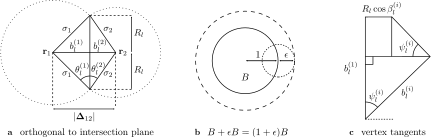
\includegraphics[width=0.9\linewidth,center]{minkowski-addition}
%%   \caption[Minkowski addition and difference]{
%%     Minkowski addition and difference.
%%     Note how these are not inverse operations.}
%% \end{SCfigure}

%% \vspace{0.5em}
%% \begin{tcolorbox}[title=Steiner's formula for parallel volumes]
%%   For a compact, convex body $K \in \mathcal{K}^d$ the parallel volume is expressable as:
%%   \begin{equation}
%%     V_d[K + \epsilon \ball_d] =
%%     \sum_{i=0}^d V_i[K] \omega_{d-i} \epsilon^{d-i}
%%   \end{equation}
%% \end{tcolorbox}

\subsection{Kinematic formulae}
\label{sec:kinematic-formula}

Here we introduce the \emph{kinematic formulae} which calculate the probabilities that uniformly distributed objects collide.
This problem is applicable to the evaluation of partition functions in statistical mechanics, of which we will see specific examples in section \ref{sec:fmt} and chapter \ref{chapter:resummation}.

Two compact and convex objects $K_1, K_2 \in \mathcal{K}^d$ overlap if their intersection is non-empty $K_1 \cap K_2 \ne \emptyset$.
The intersection of convex objects is also convex, so from the definition of the Euler characteristic \eqref{eq:euler-characteristic-definition} we can write
\begin{equation*}
  \chi[K_1 \cap K_2]
  =
  \begin{cases}
    1 & \textrm{ if } K_1 \cap K_2 \ne \emptyset \\
    0 & \textrm{ if } K_1 \cap K_2 = \emptyset
  \end{cases}
\end{equation*}
then the probability that the two objects collide is
\begin{equation*}
  \mathrm{Prob} \left[ \textrm{collision} \right]
  =
  \frac{1}{V} \int_V \chi[K_1 \cap K_2(\vec{r})] \, d\vec{r}
\end{equation*}
where $K_2$ is uniformly distributed and $K_1$ acts as a fixed target.
Here, $K_2$ is \emph{translated} over the accessible volume, however in general these objects will be non-spherical so we should also consider the \emph{rotations}.
Integral geometry more naturally deals with integrations over relative positions \emph{and} orientations, at the small cost of additional notation.
%In addition to integrations over particle positions $\{\vec{r}_1, \cdots, \vec{r}_n\}$ we also have to consider their orientations $\{\vec{\theta}_1, \cdots, \vec{\theta}_n\}$ where each $\vec{\theta}_i$ represents an Euler angle tuple.
%Then, assuming an isotropic phase where all orientations are equally likely each positional integral generalises to
Writing the relative orientation as the Euler angle tuple $\vec{\theta}$, we consider the generalisation
\begin{equation*}
  \int_{\mathbb{R}^d} d\vec{r}
  \to
  \int_{\mathbb{R}^d \times \mathrm{SO}(d)} d\vec{r} d\vec{\theta}
  :=
  \int_{G_d} dg,
\end{equation*}
with the normalisation in the angular measure such that $\int d\vec{\theta} = 1$.
In the right-most equality we introduced the rigid-motion operation acting on a body $K \in \mathcal{K}^d$ as
\begin{equation*}
  g K := \{\mathcal{R}_\theta \, \vec{k} + \vec{r} \, | \, \vec{k} \in K\},
  %(\mathcal{T} \circ \mathcal{R})(\vec{r}, \vec{\theta}),
\end{equation*}
a member of the rigid-motion group $g \in G_d := \mathbb{R}^d \times \mathrm{SO}(d)$, and where $\mathcal{R}_\theta \in \mathrm{SO}(d)$%
\marginfootnote{$\mathrm{SO}(d)$ is the \emph{special orthogonal group}, i.e.\ the group of all orthogonal matrices with unit determinant.}
is the rotation matrix parameterised by $\vec{\theta}$.
Then the generalised measure for particle collisions becomes
\begin{equation*}
  \int_{G_d} \chi[K_1 \cap g K_2] \, dg
\end{equation*}
if they occupy all of Euclidean space.
We will see integrals like this emerge from liquid state theory in sections \ref{sec:virial-series} and \ref{sec:fmt}, and later in chapter \ref{chapter:resummation}.

\vspace{0.5em}

\begin{tcolorbox}[title=Principal kinematic formula]
  %% Noting that $\chi = V_0$ is the lowest order intrinsic volume, the latter line of \eqref{eq:low-density-insertion} is ideally suited to a treatment within integral geometry.
  A central result of integral geometry is the principal kinematic formula of Blaschke and Santal\'o \cite{BlaschkeMZ1936,Blaschke1937,SantaloASI1936} which gives the explicit form of these collisional integrals as \cite{Santalo2004,Klain1997}
  %\cite{Santalo2004,SchneiderACIG1984,Schneider2008,Klain1997}
  \begin{equation}\label{eq:binomial-kinematic-formula}
    \int_{G_d} \chi[K_1 \cap g K_2] \, dg
    =
    \sum_{k=0}^d (C_{k,d-k})^{-1} V_k[K_1] V_{d-k}[K_2]
  \end{equation}
  We see the flag coefficients \eqref{eq:flag-coefficients} play an analogous role here in conjugating the intrinsic volumes as binomial coefficients do in algebraic expansions%
  \marginfootnote{For this reason Klain and Rota argue that integral geometry should be called \emph{continuous combinatorics} \cite{Klain1997}, because it generalises combinatorial results to continuous spaces}.
  More general formulae exist for integrals over $V_k[K_1 \cap K_2]$ for all $k$ \cite{Klain1997}, however these do not have an interpretation in terms of evaluating partition functions so we will not be using them.
\end{tcolorbox}

The principal kinematic formula \eqref{eq:binomial-kinematic-formula} can be iterated for the intersections of many bodies $\{K_1, \cdots, K_n\}$ giving \cite{Santalo2004,MarechalPRE2014}
\begin{subequations}\label{eq:multinomial-kinematic-formula}
  \begin{equation}
    \begin{split}
      & \quad
      \int_{G_d^n} \chi[K_1 \cap g_2 K_2 \cap \cdots \cap g_n K_n]
      \, dg_2 \cdots dg_n
      \\ = &
      \sum_{\substack{i_1, \cdots, i_n = 0 \\ i_1 + \cdots + i_n = nd}}^d
      (C_{i_1, \cdots, i_n})^{-1}
      V_{i_1}[K_1]
      \prod_{j=2}^n
      V_{i_j}[K_j],
    \end{split}
  \end{equation}
  \begin{equation}
    \textrm{with} \qquad
    C_{i_1, \cdots, i_n}
    := \frac{1}{i_1! \omega_{i_1}}
    \prod_{j=2}^n
    \left(
    \frac{d!}{i_j!} \frac{\omega_d}{\omega_{i_j}}
    \right),
  \end{equation}
\end{subequations}
where $\int_{G_d^n} dg^n = \int_{G_d} dg_1 \cdots \int_{G_d} dg_n$.
Here $C_{i_1, \cdots, i_n}$ would be the multinomial generalisation of the flag coefficients \eqref{eq:flag-coefficients}.
We will use this iterated formula in chapter \ref{chapter:resummation} to resum a piece of the virial series (to be introduced in the upcoming section \ref{sec:virial-series}).

%% We have the invariant measure on 1-dimensional linear subspaces of $\mathbb{R}^d$ (\emph{Grassmanians}) as
%% \begin{equation}
%%   [d] = \tau_d(\textrm{Gr}(d,1))
%%   = \frac{d \omega_d}{2 \omega_{d-1}}.
%% \end{equation}
%% Factorial defined as
%% \begin{equation}
%%   [k]! = \prod_{i=0}^k \, [i]
%% \end{equation}
%% Flag coefficients from binomial coefficients
%% \begin{equation}
%%   {d \brack k}
%%   := \frac{[n]!}{[k]! [n-k]!}
%%   = {d \choose k}
%%   \frac{\omega_d}{\omega_k \omega_{d-k}}
%% \end{equation}
%% Provides the generalisation of combinatorial results to continuous spaces.
%% Analagously to binomial coefficients, the flag coefficients obey
%% \begin{equation}\label{eq:flag-coefficients-symmetry}
%%   {d \brack k} = {d \brack d - k}.
%% \end{equation}
%% Note that we can rewrite \eqref{eq:intrinsic-volume-ball} using the flag coefficients as
%% \begin{equation}\label{eq:intrinsic-volume-ball-flag}
%%   \mu_k (\ball_d) = {d \choose k} \frac{\omega_d}{\omega_{d-k}}
%%   = {d \brack k} \omega_k
%% \end{equation}

%% \begin{center}
%% \begin{tabular}{cccccc}
%%   \toprule
%%   $k$ & $\omega_k$ & $[k]$ & $[k]!$ & ${2 \brack k}$ & ${3 \brack k}$ \\
%%   \midrule
%%   0 & 1 & 1 & 1 & 1 & 1 \\
%%   1 & 2 & 1 & 1 & $\frac{\pi}{2}$ & 2 \\
%%   2 & $\pi$ & $\frac{\pi}{2}$ & $\frac{\pi}{2}$ & 1 & 2 \\
%%   3 & $\frac{4\pi}{3}$ & 2 & $\pi$ & & 1 \\
%%   \bottomrule
%% \end{tabular}
%% \end{center}

%% \vspace{0.5em}
%% \begin{tcolorbox}[title=General kinematic formula]
%%   For $0 \le k \le d$:
%%   \begin{equation}
%%     \int_{\mathbb{E}_d} \mu_k (A \cap g B) \, dg =
%%     \sum_{i=0}^{d-k}
%%     {i + k \brack k} {d \brack i}^{-1}
%%     \mu_{i+k}(A) \mu_{d-i}(B)
%%   \end{equation}
%%   \begin{equation*}
%%     \int_{\mathbb{E}_d} \mu_k (A \cap g B) \, dg =
%%     \sum_{i=0}^{d-k}
%%     {i + k \brack k}
%%     {d \brack i + k}
%%     \kappa_{i+k}(A) \kappa_{d-i}(B)
%%   \end{equation*}
%%   In regular binomial:
%%   \begin{equation*}
%%     \int_{\mathbb{E}_d} \mu_k (A \cap g B) \, dg =
%%     \sum_{i=0}^{d-k}
%%     {i + k \choose k} {d \choose i}^{-1}
%%     \frac{\omega_{i+k} \omega_{d-i}}{\omega_k \omega_d}
%%     \mu_{i+k}(A) \mu_{d-i}(B)
%%   \end{equation*}
%% \end{tcolorbox}

%% \begin{equation*}
%%   {n \choose k} {k \choose p}
%%   =
%%   \frac{n!}{k!(n-k)!}
%%   \frac{k!}{p!(k-p)!}
%%   =
%%   \frac{n!}{p!(k-p)!(n-k)!}
%%   =
%%   {n \choose p, k-p, n-k}
%% \end{equation*}
%% I.e. this is a trinomial coefficient.
%% So we have
%% \begin{equation*}
%%   {n \brack k} {k \brack p}
%%   =
%%   {n \choose k}
%%   {k \choose p}
%%   \frac{\omega_n}{\omega_k \omega_{n-k}}
%%   \frac{\omega_k}{\omega_p \omega_{k-p}}
%%   =
%%   {n \choose p, k-p, n-k}
%%   \frac{\omega_n}{\omega_p \omega_{k-p} \omega_{n-k}}
%% \end{equation*}
